A single film does not have the necessary interactions to fulfill the neutron count rate criteria multiple films are necessary, and the arrangement of these films provides a design space for a replacement RPM.
In the case of the RPM, there are several design parameters that can be explored:
\begin{itemize}
  \item the neutron absorber loading of the film,
  \item the thickness of the film,
  \item the geometry of the film (cylinders or sheets), and
  \item the placement of the films.
\end{itemize}
It is expected that the loading of the film will be limited by the optical clarity, and that the thickness of the film will be determined by the optimization of the energy deposition.
Thus, of the above design parameters only the geometric placement of the films is an available optimization space.

Preliminary work by this author provided a simple design in which the detector layers are linearly placed throughout the detector volume in an alternating fashion.
The analysis of the neutron flux throughout this detector lead to a flat flux profile as shown in \autoref{fig:AltLayerThermalNeutronFraction}.
\begin{figure}
  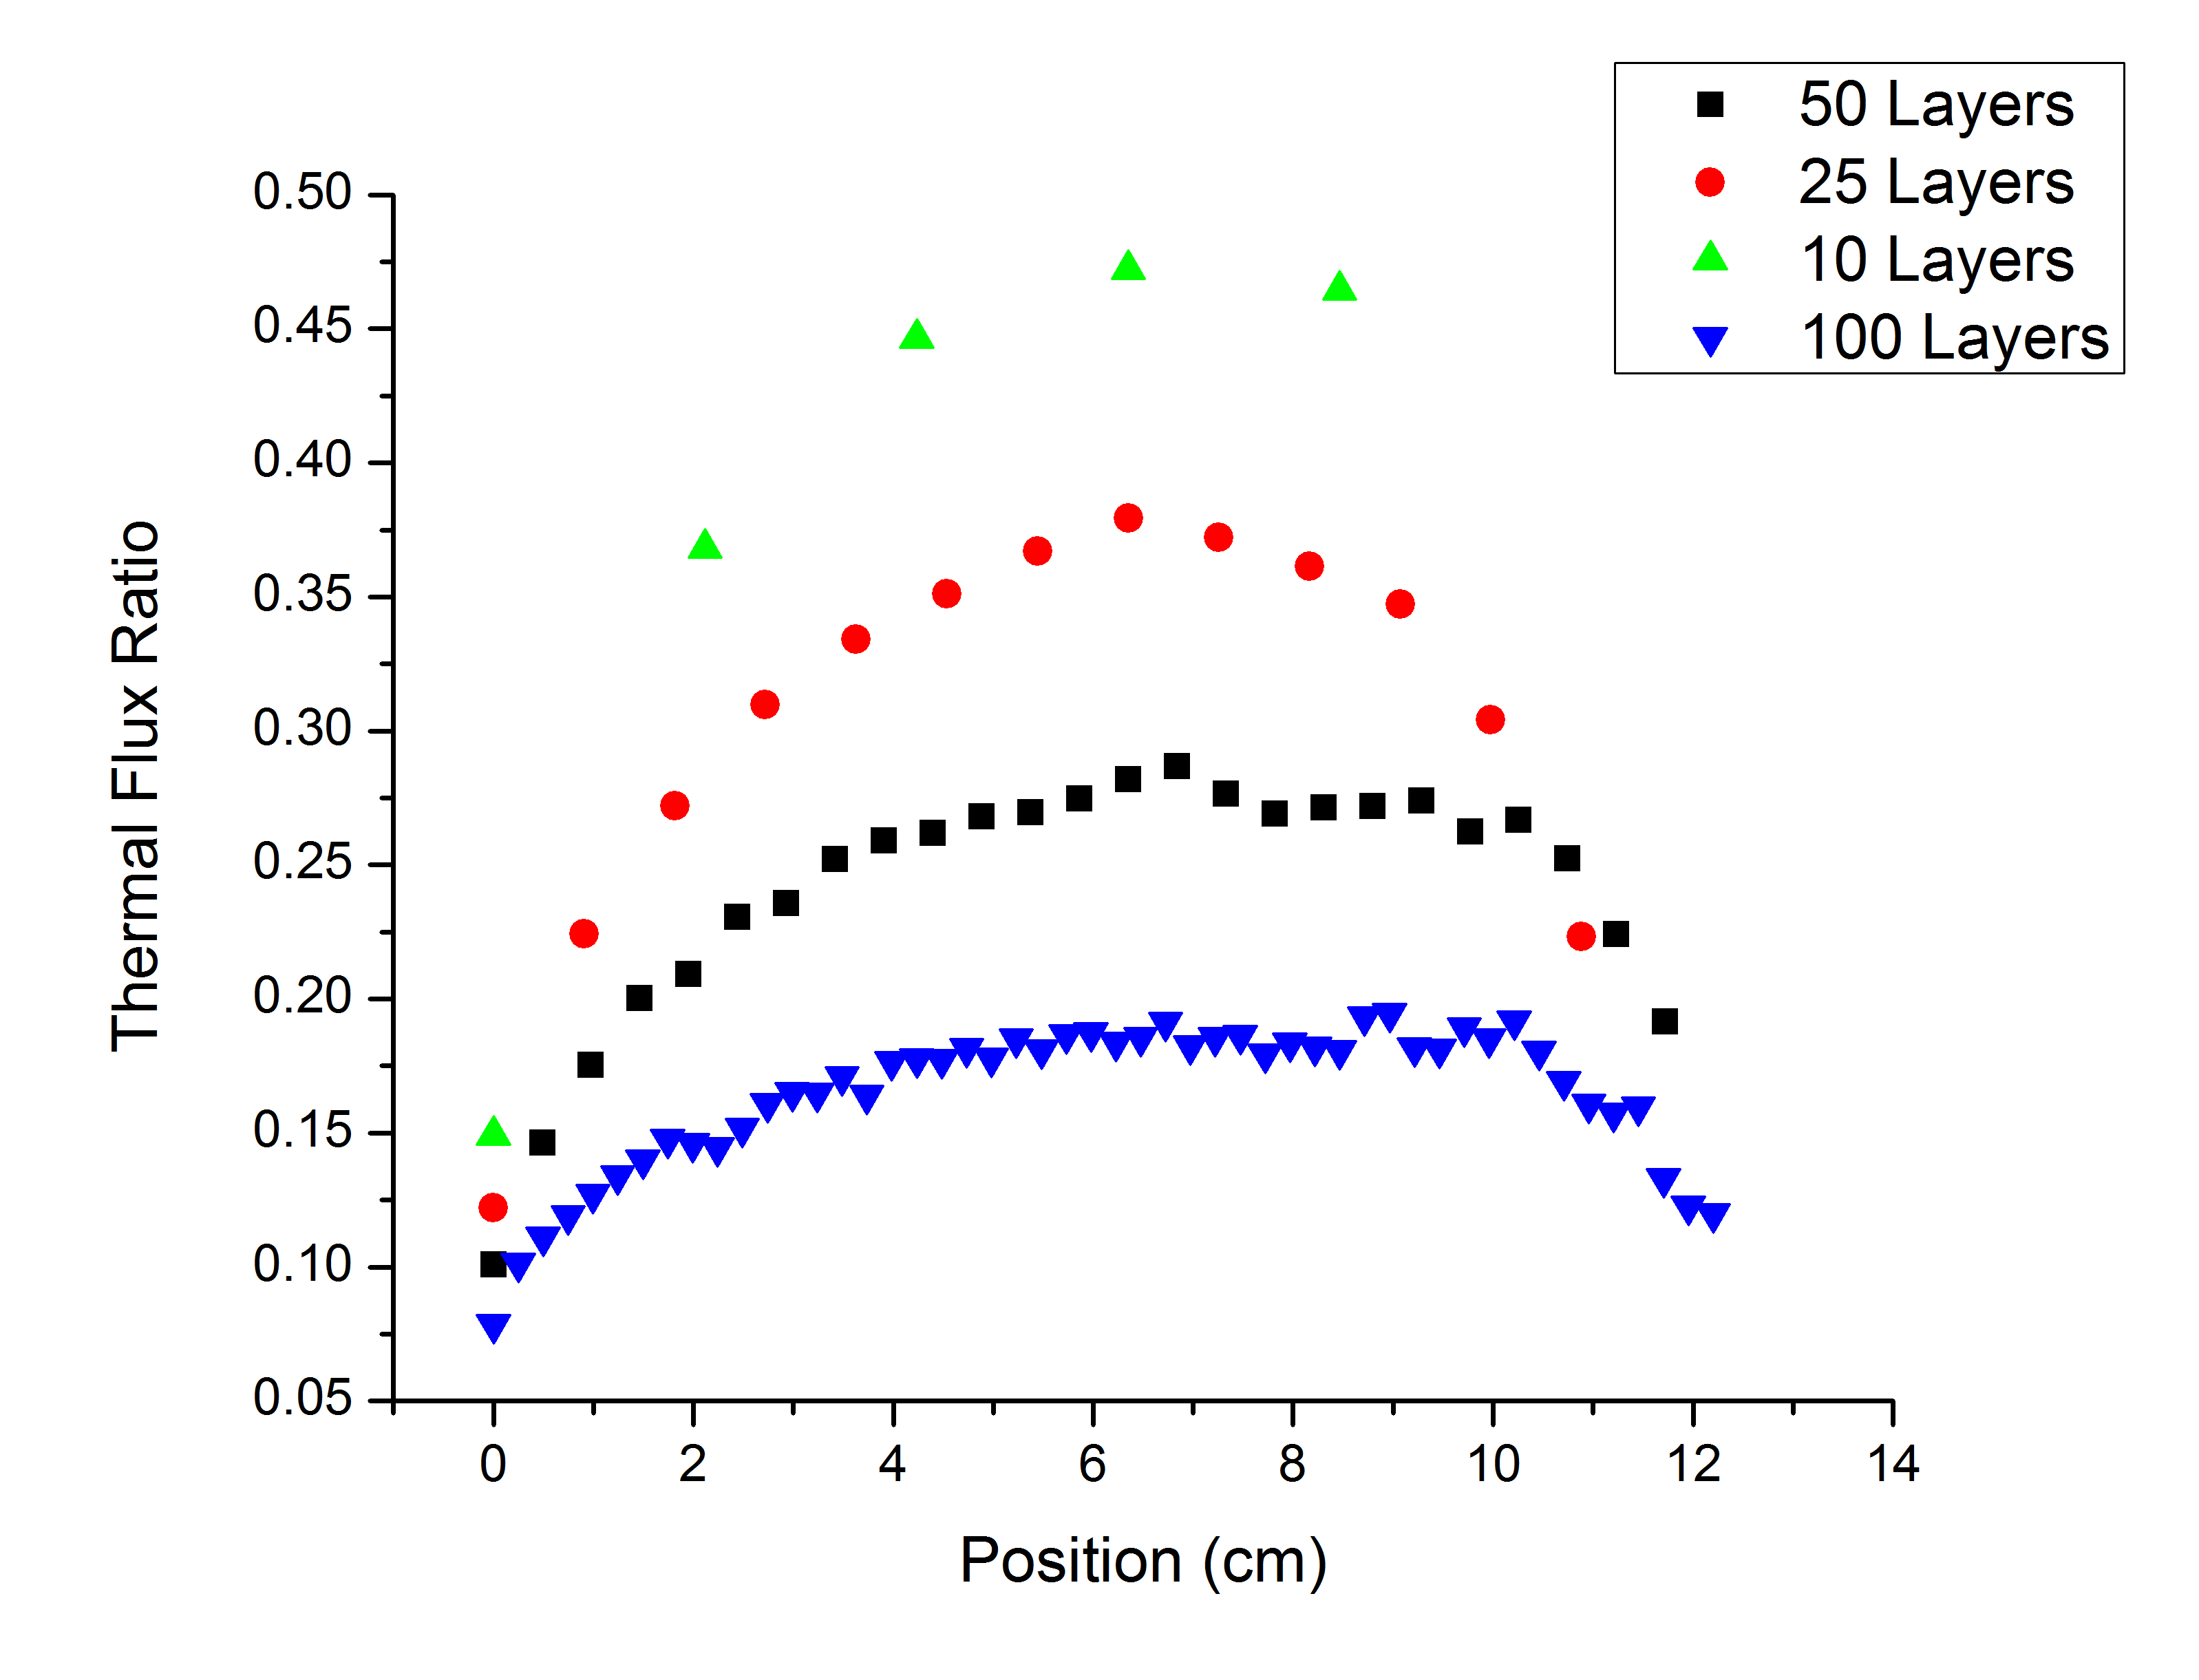
\includegraphics[width=\textwidth]{ThermalFluxRatioAltLayers}
	\caption{Fraction of the neutron flux that is thermalized through a alternating detector and moderator layered RPM.  The low thermal fluxes result in a poor utilization of the high thermal cross section of \iso[6]{Li}.}
	\label{fig:AltLayerThermalNeutronFraction}
\end{figure}
Effective utilization of the neutron flux is necessary for minimizing the amount of neutron absorber (\iso[6]{Li}) that is used in the detector.
Several different strategies can then be used to optimize the geometry to ensure effective utilization of the thermal cross section of the absorber material.

\section{Optimal Detector Geometries}

\subsection{XSDRN and MCNPX Model Comparison}
The comparison between the MCNPX simulation and the XSDRN is shown for some of the samples in \autoref{tab:10GenomeXSDRNMCNPXCompare} and \autoref{tab:20GenomeXSDRNMCNPXCompare}, where the change in rank is computed by rank of the MCNPX model versus the rank of the XSDRN model.
It is observed that the XSDRN model preformed faily closesly to the MCNPX model, but tended to over predict and favor geometries that had repeated layers and clusters.
\begin{table}
  \caption[10 Genome Length RPM Model]{10 Genome Length RPM Model Interactions rates}
  \label{tab:10GenomeXSDRNMCNPXCompare}
  \begin{tabular}{c c | c c | c}
    \toprule
    XSDRN Model & Activity & MCNPX Model & Interaction Rate & Rank Change \\
    \midrule
  0111000000 & 10.95 & 0101010000 &  3.08 & $\downarrow$ 10 \\
  0110100000 & 10.50 & 0101100000 &  2.93 & $\uparrow$ 2 \\
  0110010000 & 10.21 & 0110010000 &  2.89 & 0 \\
  0101100000 & 10.12 & 0110100000 &  2.85 & $\downarrow$ 2 \\
  0111100000 & 13.16 & 0110001000 &  2.84 & $\downarrow$ 4 \\
    \bottomrule
  \end{tabular}
\end{table}
\begin{table}
  \caption[20 Genome Length RPM Model]{20 Genome Length RPM Model Interactions rates}
  \label{tab:20GenomeXSDRNMCNPXCompare}
  \begin{tabular}{c c | c c | c}
    \toprule
    XSDRN Model & Activity & MCNPX Model & Interaction Rate & Rank Change \\
    \midrule
  01111000000000000000 & 30.39 & 00110010000000000000 &  3.14 & $\downarrow$ 10 \\
  01111100000000000000 & 23.93 & 01010010000000000000 &  3.14 & $\downarrow$ 7 \\
  01011010010000000000 & 23.46 & 01011000000000000000 &  2.65 & $\downarrow$ \\
  01111010010000000000 & 27.14 & 01101000000000000000 &  2.60 & $\downarrow$ 5\\
  01111000000000100000 & 20.22 & 01011010010000000000 &  4.29 & $\uparrow$ 2\\
    \bottomrule
  \end{tabular}
\end{table}

\subsection{Pertubations on the MCNPX Model}
Perturbations on the MCNPX were preformed in order to determine if a minimum in the search function was achieved.
For the ten length genomes where each slice is \SI{1.27}{\cm} and a perturbation moves a slice \SI{6.35}{\mm} it is observed that perturbations increase the count rate by 15\%.




A physical basis of the optimal solution found by the genetic algorithm can be found by observing the form of the optimal solutions.
These solutions involve an initial moderator layer in order to ensure that all of the neutrons are thermalized to (increasing the thermal fraction by \textbf{SOME PERCENT}).
After this moderator layer a film layer is placed to utilize this neutron spectra; however not all of the thermal neutrons are captured (as the mean free path of a neutron in polyethylene is about \SI{0.37}{\cm} and thus some pass through the material) and another absorber layer is needed to capture those neutrons.  
The neutron flux is then moderated again, and additional layers of detectors are needed to capture this neutron cross section.
However, it is desirably to have a large neutron reflector in the portal monitor to reflect neutrons back into the detector slices. 
Theoretically this reflector should be as large as possible, but the limited space of the RPM provides a constraint.
A parameter study with a single detector slice between a moderator and reflector constrained by the radiation portal monitor design showed that it is desirable to have around \textbf{So much} moderator leaving the majority of the RPM to be left for the reflector.
Thus it is demonstrated that a large reflector is desired.